\capitulo{3}{Conceptos teóricos}

\section{Conceptos sobre \textit{League of Legends}}

\subsection{El juego}
\textit{League of Legends} es un videojuego de estrategia multijugador del tipo \textit{MOBA (Multiplayer Online Battle Arena)} lanzado en 2011 en el que dos equipos de cinco jugadores se enfrentan para destruir la base del equipo enemigo \cite{misc:como-jugar}. Cada jugador controla dentro del juego a un personaje llamado campeón, que pueden seleccionar antes de empezar a jugar, y es único entre los diez jugadores.

Los jugadores se enfrentan en un mapa \ref{fig:mapa-lol} en forma de cuadrado, con las bases de cada equipo localizadas zonas opuestas del mapa, una en la esquina inferior izquierda, y la otra en la superior derecha. Conectando cada base se encuentran tres líneas o calles, superior o \textit{top}, central o \textit{mid} e inferior o \textit{bot}. El espacio entre las calles se denomina jungla. Conectando las dos esquinas que no pertenecen a las bases se encuentra el río, que se encarga de separar el terreno del mapa dominado por cada equipo. De forma general los jugadores se reparten de la siguiente manera, uno en \textit{top}, uno en \textit{mid}, dos en \textit{bot} y el restante en la jungla.

\begin{figure}
	\centering
	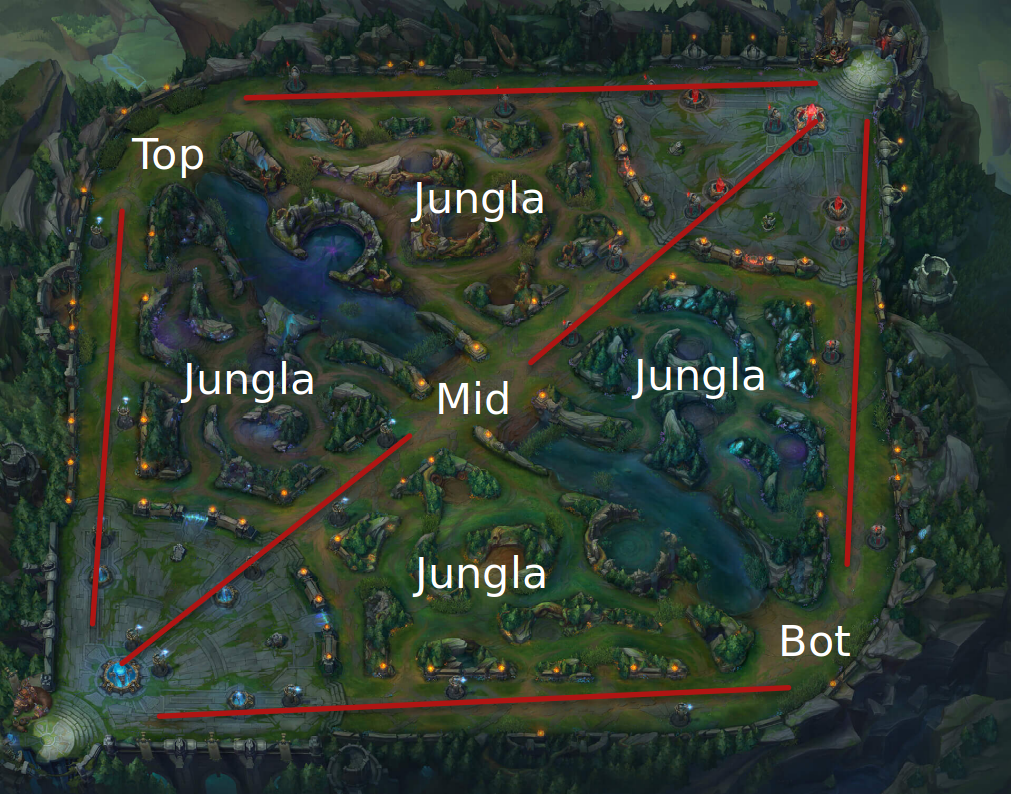
\includegraphics[width=1\linewidth]{img/mapa-lol}
	\caption{Mapa de League of Legends}
	\label{fig:mapa-lol}
\end{figure}

Para ganar la partida hay que destruir el nexo del equipo enemigo, es la estructura que está más alejada de la base propia. Está protegido por otro tipo de estructuras llamadas torres, que se encargar de proteger las calles de cada equipo y el nexo. Existen tres torres por cada línea y equipo, y dos adicionales que se encargan de proteger el nexo. Las torres se tienen que derribar en el orden que se van encontrando en cada línea, no se puede destruir directamente el nexo si, como mínimo, no se han destruido todas las torres de una calle del equipo rival.

La forma en la que un equipo consigue ventaja sobre el rival es mediante el oro, este se consigue de varias formas. La principal forma es asesinando a los campeones enemigos. Otra formas de conseguir oro es destruyendo las estructuras enemigas. La última forma de conseguir oro es matando monstruos y súbditos, los primeros se encuentras en la jungla, los segundos recorren las calles en oleadas. Tanto los campeones como los monstruos y súbditos vuelven a aparecen pasado un tiempo concreto, las estructuras una vez destruidas se mantienen así.

El oro permite comprar objetos, que mejoran las habilidades del campeón, haciendo que sea más sencillo derrotar a los campeones enemigos, lo que proporciona más oro para más objetos, causando un efecto bola de nieve y la eventual victoria del equipo.

Para ver estos conceptos de una forma más visual, Riot Games preparó un vídeo informativo de cara a los mundiales de 2020 para que la gente que no tuviera mucho conocimiento del juego y su funcionamiento pudiera ver y disfrutar la competición. El vídeo se titula \href{https://www.youtube.com/watch?v=ERkt_1TYlkU}{¿Así que queréis ver el Mundial? | Mundial 2020 - League of Legends}\footnote{\url{https://youtu.be/ERkt_1TYlkU}} y se encuentra disponible en YouTube.


\subsection{Campeones}
Los campeones son los diferentes personajes disponibles que un jugador puede seleccionar antes de la partida. Actualmente hay 156 disponibles, añadiéndose a la lista uno nuevo en franjas de tiempo que van desde uno a seis meses. Cada uno tiene un rol asignado que determina su forma de jugar, su función e incluso posición dentro del mapa.
\begin{itemize}
	\tightlist
	\item Tirador
	\item Apoyo
	\item Asesino
	\item Luchador
	\item Tanque
	\item Mago
\end{itemize}

Para que un campeón acabe en una categoría u otra hay que prestar atención a varios factores, entre los que se encuentran su tipo de ataque básico, el efecto de sus habilidades y la forma en la que sus estadísticas modifican las habilidades. En las secciones \ref{habilidades} y \ref{estadisticas} se explican en detalles estos conceptos.

\subsection{Habilidades}
\label{habilidades}
Cada campeón tiene un conjunto único de habilidades, una pasiva y cuatro activas. Se pueden definir con las operaciones que un jugador puede realizar para interactuar dentro de la partida con el mapa, otros jugadores, monstruos y súbditos.

Cada habilidad puede tener un efecto o combinar varios, los cuales se aplican sobre uno mismo, un aliado o enemigo. Los efectos más comunes son las curaciones, realizar daños o control de adversario, donde se engloban ralentizaciones o inmovilizaciones. Estos efectos tienen unos valores numéricos que constan de dos partes, un valor base y uno variable que depende de las estadísticas del campeón.

En el caso de realizar daño a un rival, existen tres formas en que las que puede realizar: daño físico, mágico o verdadero. Esto está determinado por la habilidad y rol del campeón.

\subsection{Estadísticas}
\label{estadisticas}
Las estadísticas son diferentes valores numéricos que determinan las capacidades de cada campeón en un área en concreto del juego. Estos valores se ven modificados por la compra de objetos (\ref{objetos}). A continuación se describen las estadísticas y que representan.
\begin{description}
	\item[Daño de ataque] Daño realizado con ataques básicos.
	\item[Probabilidad de crítico] Probabilidad de que un ataque básico haga el doble de daño.
	\item[Velocidad de ataque] Cantidad de ataques básicos que se pueden realizar por segundo.
	\item[Poder de habilidad] Modifica el daño que realizan las habilidades.
	\item[Velocidad de movimiento] Velocidad a la que un campeón se desplaza por el mapa.
	\item[Armadura] Protección frente al daño físico.
	\item[Resistencia mágica] Protección frente al daño mágico.
	\item[Penetración de armadura] Omisión de la armadura del rival.
	\item[Penetración mágica] Omisión de la resistencia mágica del rival.
	\item[Vida] Daño que tiene que recibir un personaje para morir.
	\item[Maná] Coste de usar habilidades.
	\item[Robo de vida] Porcentaje de vida recuperado al dañar a un rival.
\end{description}

\subsection{Objetos}
\label{objetos}
Dentro de la base de cada equipo en el mapa está localizada la tienda. Aquí los jugadores pueden comprar objetos con el oro que han ido ganando con el progreso de la partida. Su función es modificar las estadísticas del campeón, para que las habilidades del mismo sean más eficaces contra los rivales. Los objetos que se comprar se quedan guardados en el inventario del campeón, el cual está limitado a seis objetos.

En el juego actual existen 222 objetos disponibles clasificados en cinco categorías.
\begin{description}
	\item[Iniciales] Objetos más relevantes al inicio de la partida.
	\item[Básicos] Objetos que mejoran una estadística.
	\item[Épicos] Objetos formados por la combinación de varios objetos básicos que mejoran varias estadísticas.
	\item[Legendarios] Objetos formados por la combinación de objetos épicos y/o básicos que mejoran varias estadísticas y proporcionan algún efecto adicional.
	\item[Míticos] Igual que los anteriores, pero limitado a uno en el inventario.
\end{description}


\subsection{Ligas}






En aquellos proyectos que necesiten para su comprensión y desarrollo de unos conceptos teóricos de una determinada materia o de un determinado dominio de conocimiento, debe existir un apartado que sintetice dichos conceptos.

Algunos conceptos teóricos de \LaTeX \footnote{Créditos a los proyectos de Álvaro López Cantero: Configurador de Presupuestos y Roberto Izquierdo Amo: PLQuiz}.

\section{Secciones}

Las secciones se incluyen con el comando section.

\subsection{Subsecciones}

Además de secciones tenemos subsecciones.

\subsubsection{Subsubsecciones}

Y subsecciones.


\section{Referencias}

Las referencias se incluyen en el texto usando cite \cite{wiki:latex}. Para citar webs, artículos o libros \cite{koza92}.


\section{Imágenes}

Se pueden incluir imágenes con los comandos standard de \LaTeX, pero esta plantilla dispone de comandos propios como por ejemplo el siguiente:

\imagen{escudoInfor}{Autómata para una expresión vacía}



\section{Listas de items}

Existen tres posibilidades:

\begin{itemize}
	\item primer item.
	\item segundo item.
\end{itemize}

\begin{enumerate}
	\item primer item.
	\item segundo item.
\end{enumerate}

\begin{description}
	\item[Primer item] más información sobre el primer item.
	\item[Segundo item] más información sobre el segundo item.
\end{description}

\begin{itemize}
\item
\end{itemize}

\section{Tablas}

Igualmente se pueden usar los comandos específicos de \LaTeX o bien usar alguno de los comandos de la plantilla.

\tablaSmall{Herramientas y tecnologías utilizadas en cada parte del proyecto}{l c c c c}{herramientasportipodeuso}
{ \multicolumn{1}{l}{Herramientas} & App AngularJS & API REST & BD & Memoria \\}{
HTML5 & X & & &\\
CSS3 & X & & &\\
BOOTSTRAP & X & & &\\
JavaScript & X & & &\\
AngularJS & X & & &\\
Bower & X & & &\\
PHP & & X & &\\
Karma + Jasmine & X & & &\\
Slim framework & & X & &\\
Idiorm & & X & &\\
Composer & & X & &\\
JSON & X & X & &\\
PhpStorm & X & X & &\\
MySQL & & & X &\\
PhpMyAdmin & & & X &\\
Git + BitBucket & X & X & X & X\\
Mik\TeX{} & & & & X\\
\TeX{}Maker & & & & X\\
Astah & & & & X\\
Balsamiq Mockups & X & & &\\
VersionOne & X & X & X & X\\
}
